\chapter{Sensors}
\label{chap:sensors}
\section{Pressure sensitive films}
Pressure-sensitive films are thin sensors used to measure forces in areas where space is an issue. Thin film sensors are seen in areas where one would need to register changes in forces to a solid or flexible surface. These force sensing sensors are also referred to as Force Sensing Resistors (FSR). Pressure sensitive films and force sensing resistors are sensors whose resistance decrease with increasing applied force, thus increasing conductivity.

\subsection{Construction of the sensor}
The sensor is typically based on five layers. As shown in Figure \ref{fig:sensorconstruction}, the five layers may be the two protective films, which envelopes the sensor as a protective layer. In between the protective layers, two conductive electrodes encloses a layer of conductive ink. The electrodes allow electrons to flow through the ink from one electrode to the other.

\subsection{Construction materials}
\label{subsec:materials}
The electrodes can be produced from any conductive material. In terms of producing cheap and reliable sensors, materials like silver is used. Film materials used as protective layers, such as dielectric Polyester, are elastic and flexible to allow placement of the sensor in variuos areas. The flexible material also works as an insulator for the electrodes. The ink used to conduct electrons between the electrode plates is described to be produced by screen printing piezoresistive ink with a predefined pattern. The ink is printed as thick films having a thickness ranging from 10$\mu m$ to 40$\mu m$. The ink is later dried at \SI{150}{\celsius} and then sintered from \SI{700}{\celsius} to \SI{900}{\celsius}. The sintering makes grains of conductive and insulating oxides bind together and give them cohesion and strength. This results in the ink containing small submicron particles of various metal oxides \citep[10.3, p.418]{handbook}.

\subsection{How does the sensor register force?}
When applying force to the sensor, the conductivity increases by increasing connection between the electrodes through three main mechanisms.
The three different mechanisms are conduction, hopping and tunneling.
Based on these, the amount of electrons passing through the ink, increases with more force on the sensor. As shown in Figure \ref{fig:sensorconcept}, conduction is direct contact in the particles of the ink, this happens when the particles are fully connected. Hopping occurs when the particles are close enough to allow the electrons to jump. Typically, the jumping effect happens when the distance between the particles are around 10$nm$. The final mechanism is tunneling. This happens when the particles are barely touching (at around 1$nm$) and establishes a path for the electrons \citep[10.3, p.418]{handbook}.

\begin{figure}[!htb]
   \begin{minipage}{0.470\textwidth}
     \centering
     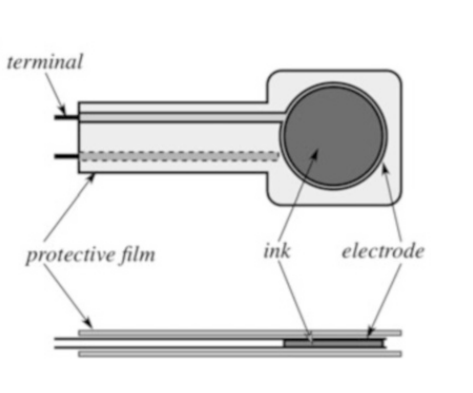
\includegraphics[width=0.8\textwidth]{figures/sensorconstruction.png}
     \caption{Composition of thin-film pressure sensor. Figure taken from \cite[p.418]{handbook}}
     \label{fig:sensorconstruction}
   \end{minipage}\hfill
   \begin{minipage}{0.475\textwidth}
     \centering
     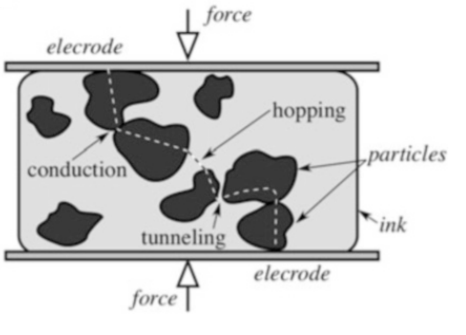
\includegraphics[width=0.9\textwidth]{figures/sensorconcept.png}
     \caption{Concept of pressure-sensitive ink. Figure taken from \cite[p.418]{handbook}}
     \label{fig:sensorconcept}
   \end{minipage}
\end{figure}

\subsection{Usage}
The sensor operates in the voltage area of the input voltage of the circuit. This can typically be from $0V$ to $+5V$. By applying force on the sensor, the resistance decreases and conductivity increases. Depending on the applied force on the sensor, the voltage output varies, allowing simple reading and measuring of the output voltage. The sensor's idle state, without load, is described to have mega-ohms of resistance. This makes the idle state difficult as a minimum value for calibration.
The circuits used are simple voltage dividers or operational amplifier circuits. Where the latter prevents the sensor to draw power directly from the circuit supply voltage.

\subsection{Measurement quality}
The pressure-sensitive sensor is often linear, in terms of conductivity versus force. Sensors like the FlexiForce A201 \ref{sec:flexiforce}, has a linearity error of $\pm$ 3\%). Due to time drift in the sensor, the ink material need time to rest after a period of measuring. The conductance increases over time \ref{fig:timedrift}. The measurements tend towards non-linear after around 60 seconds and the data is no longer usable.
Allowing of the ink to settle to ensure consistency in the results is important when gathering data \citep{vecchi_experimental_2000} with the pressure-sensitive film sensors.

\section{FlexiForce A201 Sensor}
\label{sec:flexiforce}
The FlexiForce A201 sensor from Tekscan is a pressure sensitive film, constructed of two layers of plastic substrates films like polyester. Each layer consists of a conductive material (silver), which encloses a layer of conductive ink with adhesive, as described in Section \ref{subsec:materials}. The sensing area is defined by a circular pattern of $9.8mm$, extended to two connectors for reading voltage (Figure \ref{fig:tekscana201}. Tekscan, Inc. offers three variations of the FlexiForce A201 sensor. Low$^1$ 4,4\si{\newton}, Medium$^2$ 111\si{\newton}, and High$^3$ 445\si{\newton}, where the latter can be adjusted to have a sensing area up to 4448\si{\newton} by adjusting the sensitivity in the circuit \citep{tekscanA201}.


\section{Interlink Force Sensing Resistor}
\label{sec:interlink}
The FSR from Interlink Electronics is a common device used for sensing changes in force from contact, with an optimized sensitivity for use in human touch \citep{interlinkelectronics}. The FSR sensor consists of two conductive layers with interdigitated patterns which is commonly found in heat sensors. The interdigitated layers are deposited on a thermoplastic sheet facing a conductive polyetherimide film sheet. A spacer placed between the sheets allows electrical contact when force is applied \citep{vecchi_experimental_2000}. Similar to the Flexiforce A201 sensor, this sensor also contain a circular sensing area with a diameter of $14.7 mm$ (Figure \ref{fig:fsr402}).

\begin{figure}[!htb]
   \begin{minipage}{0.45\textwidth}
     \centering
     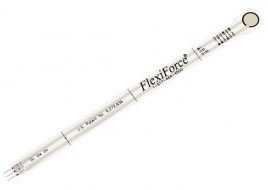
\includegraphics[width=1\textwidth]{figures/A201.jpg}
     \caption{Force sensing sensor (by Tekscan, Inc.). Figure taken from \textit{https://www.tekscan.com/products-solutions/force-sensors/a201}}
     \label{fig:tekscana201}
   \end{minipage}\hfill
   \begin{minipage}{0.45\textwidth}
     \centering
     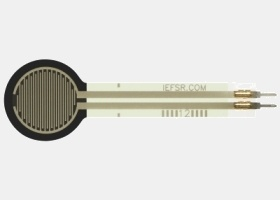
\includegraphics[width=1\textwidth]{figures/FSR-402.jpg}
     \caption{Force sensing resistor (FSR by Interlink Electronics). Figure taken from \textit{https://www.interlinkelectronics.com
     /fsr-402}}
     \label{fig:fsr402}
   \end{minipage}
\end{figure}



\section{Chapter results}
Two tests were conducted on the FlexiForce A201 sensors. The time drift test (Figure \ref{fig:timedrifttest} confirmed the characteristics of the sensor which was researched by \cite{vecchi_experimental_2000}.
The sensor gave linear results when conducting the linearity test (Figure \ref{fig:linearitytest}, with small variations. The linearity test was testing with a weight interval illustrated in Figure \ref{fig:weightinterval}.

\begin{figure*}
    \centering
    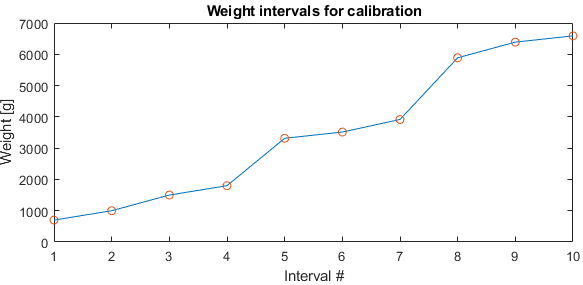
\includegraphics[width=1\textwidth]{figures/weight_interval2.png}
    \caption{Weight interval for linearity test and sensor calibration}
    \label{fig:weightinterval}
\end{figure*}
\begin{figure*}
    \centering
     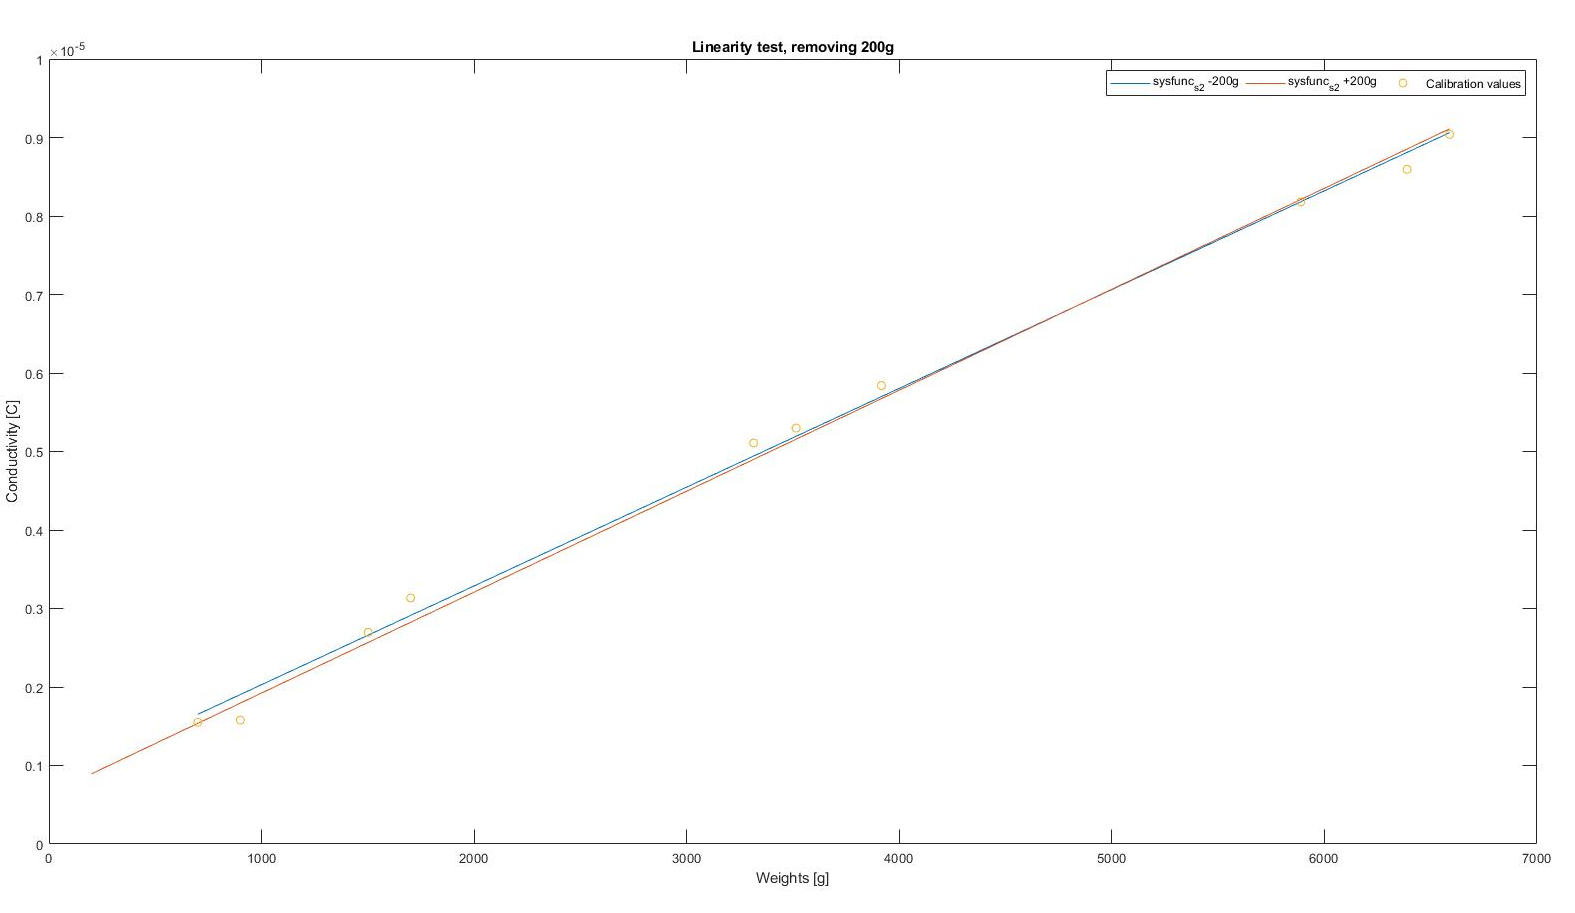
\includegraphics[width=1\textwidth]{figures/comp_sensor2.jpg}
     \caption{Linearity test of the FlexiForce A201 sensor}
     \label{fig:linearitytest}
\end{figure*}
\begin{figure*}
    \centering
     \includegraphics[width=0.9\textwidth]{figures/timedrift_test.png}
     \caption{Time drift test of the FlexiForce A201 sensor}
     \label{fig:timedrifttest}
\end{figure*}

\section{Chapter discussion}
The dimensions of the FSR sensor from Interlink Electronics did not meet the size requirements to be placed on the mechanical design (Section \ref{sec:mechanicaldesign}. FlexiForces' A201 sensor allowed two sensor to fit under the width of a cross-country ski, thus giving the ability to conduct two-dimensional measurements of a cross-country ski. Time drift test in Figure \ref{fig:timedrifttest} show an increase in conductivity under load for 30 seconds. Which in terms measurement time is a limitations that needs to be considered. The conductance stabilizes after 10 seconds which indicates the start of data collection for the FlexiForce A201 sensor. From the linearity test illustrated in Figure \ref{fig:linearitytest}, the variations in the lower spectrum of applied forces indicates a potential source of measurement error. The 100lb A201 sensor proved more stable and accurate results in the higher ranges of weight.

\section{Chapter conclusion}
Based on the researched done by \cite{vecchi_experimental_2000}, the same choice of sensors was done for this thesis after running the time drift- and linearity-tests. The FlexiForce A201 sensor met the required specifications of linearity and force limitations(0N - 245.25N). The sensor need to handle a total loading weight of 25kg (245.25N) which is based of the sensor placement with the total loaded weight on the system. The mechanical design presented in Section \ref{sec:mechanicaldesign}, divides half the FBW loaded onto each side of the system. The weight is again divided between the cross sections along the running phase of the system. Resulting in $\frac{FBW}{4}$ potential max load on a single sensor. Variations in the lower spectrum of the 100lb A201 sensor introduced an error beyond $\pm$ 3\%. A conclusion was made to discard measurement values below 700g. Values between 0g and 700g was instead used to register contact with the sensor.